\section*{Appendices}

	\begin{frame}
		\frametitle{Appendix A.1: Scenario \textrm{I} (State Trajectory Evolution)}\label{a.1}
		\centering
		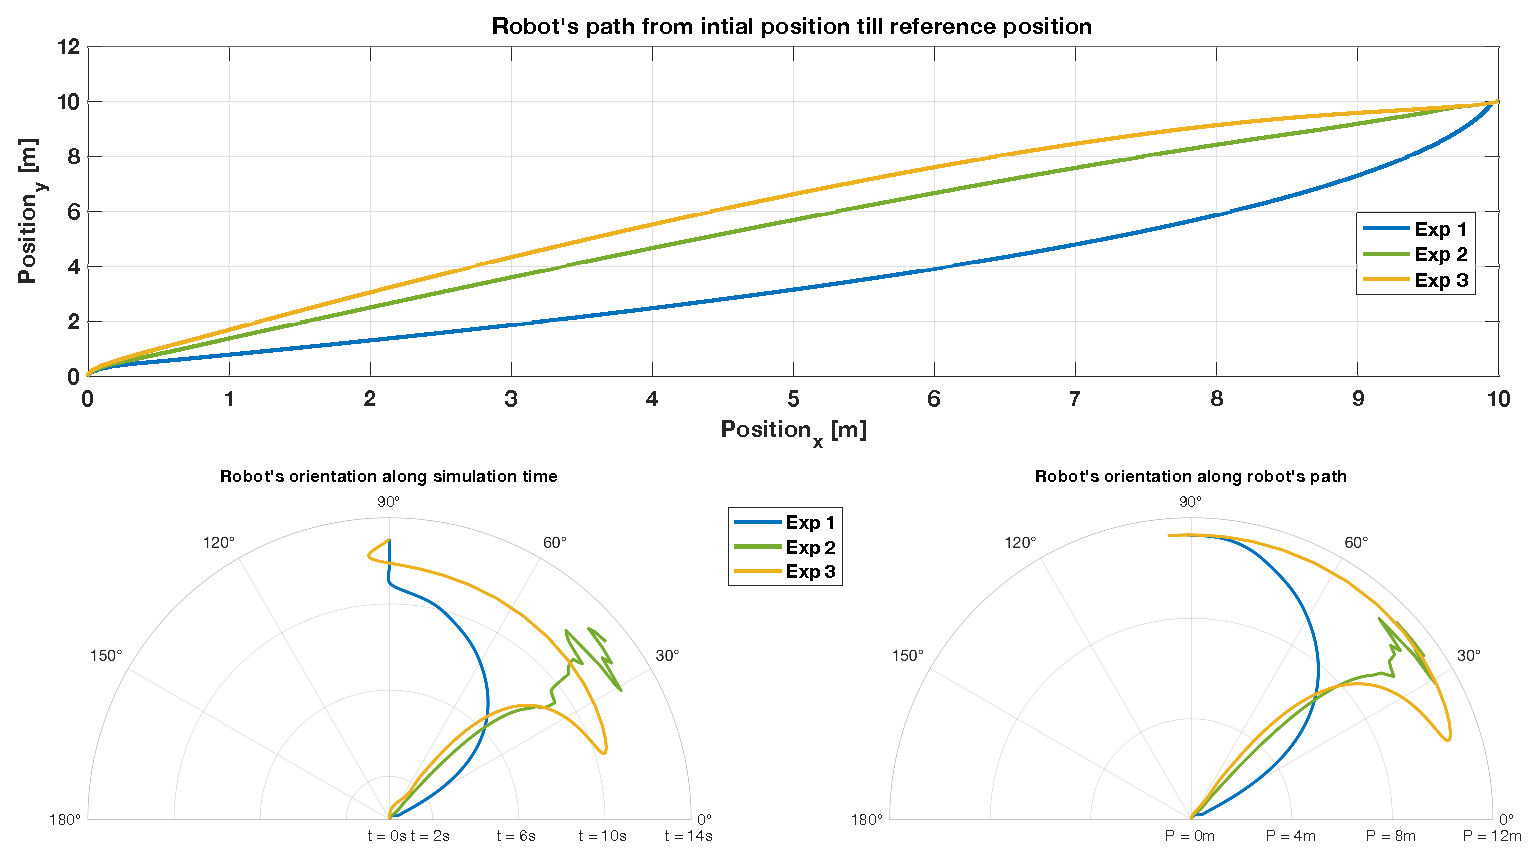
\includegraphics[scale=0.45]{pictures/graphs/sn1_states.eps}
	\end{frame}

	\begin{frame}
		\frametitle{Appendix A.2: Scenario \textrm{I} (Input Trajectory Evolution)}\label{a.2}
		\centering
		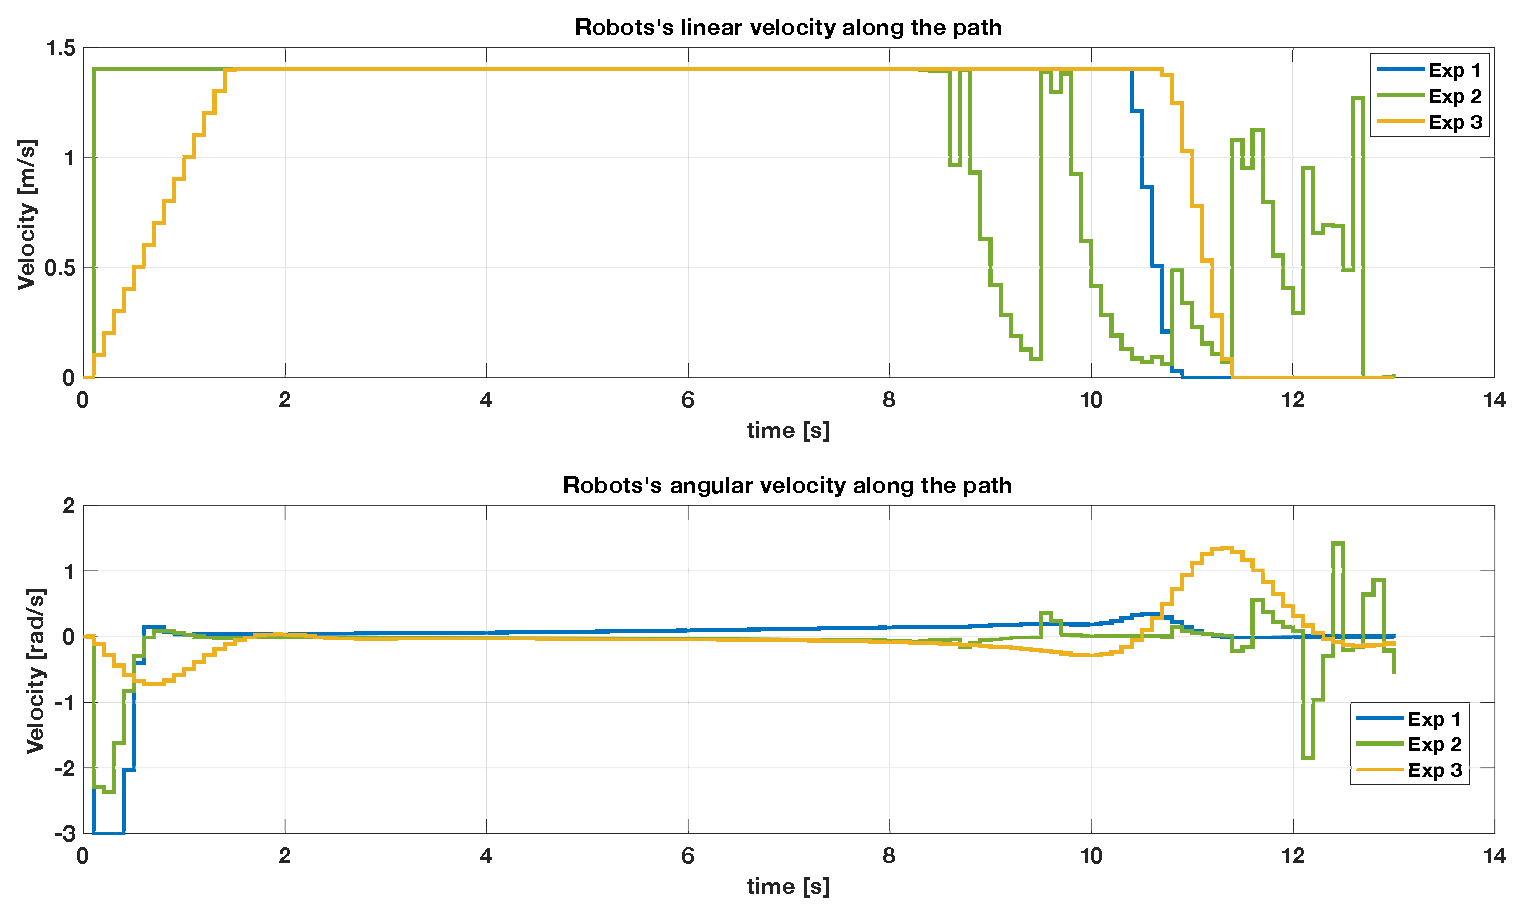
\includegraphics[scale=0.42]{pictures/graphs/sn1_inputs.eps}
	\end{frame}

	\begin{frame}
		\frametitle{Appendix A.3: Scenario \textrm{I} (NMPC Computational Effort)}\label{a.3}
		\centering
		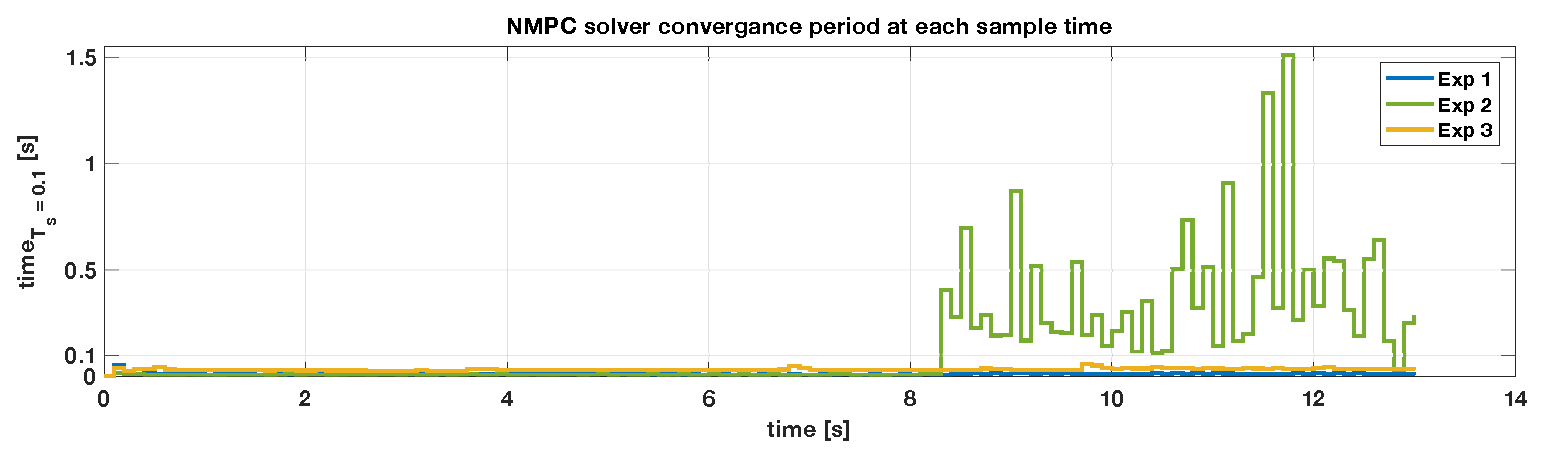
\includegraphics[scale=0.42]{pictures/graphs/sn1_solver_time.eps}
	\end{frame}
 
 	\begin{frame}
 		\frametitle{Appendix B.1: Scenario \textrm{II} (State Trajectory Evolution)} \label{b.1}
		\centering
		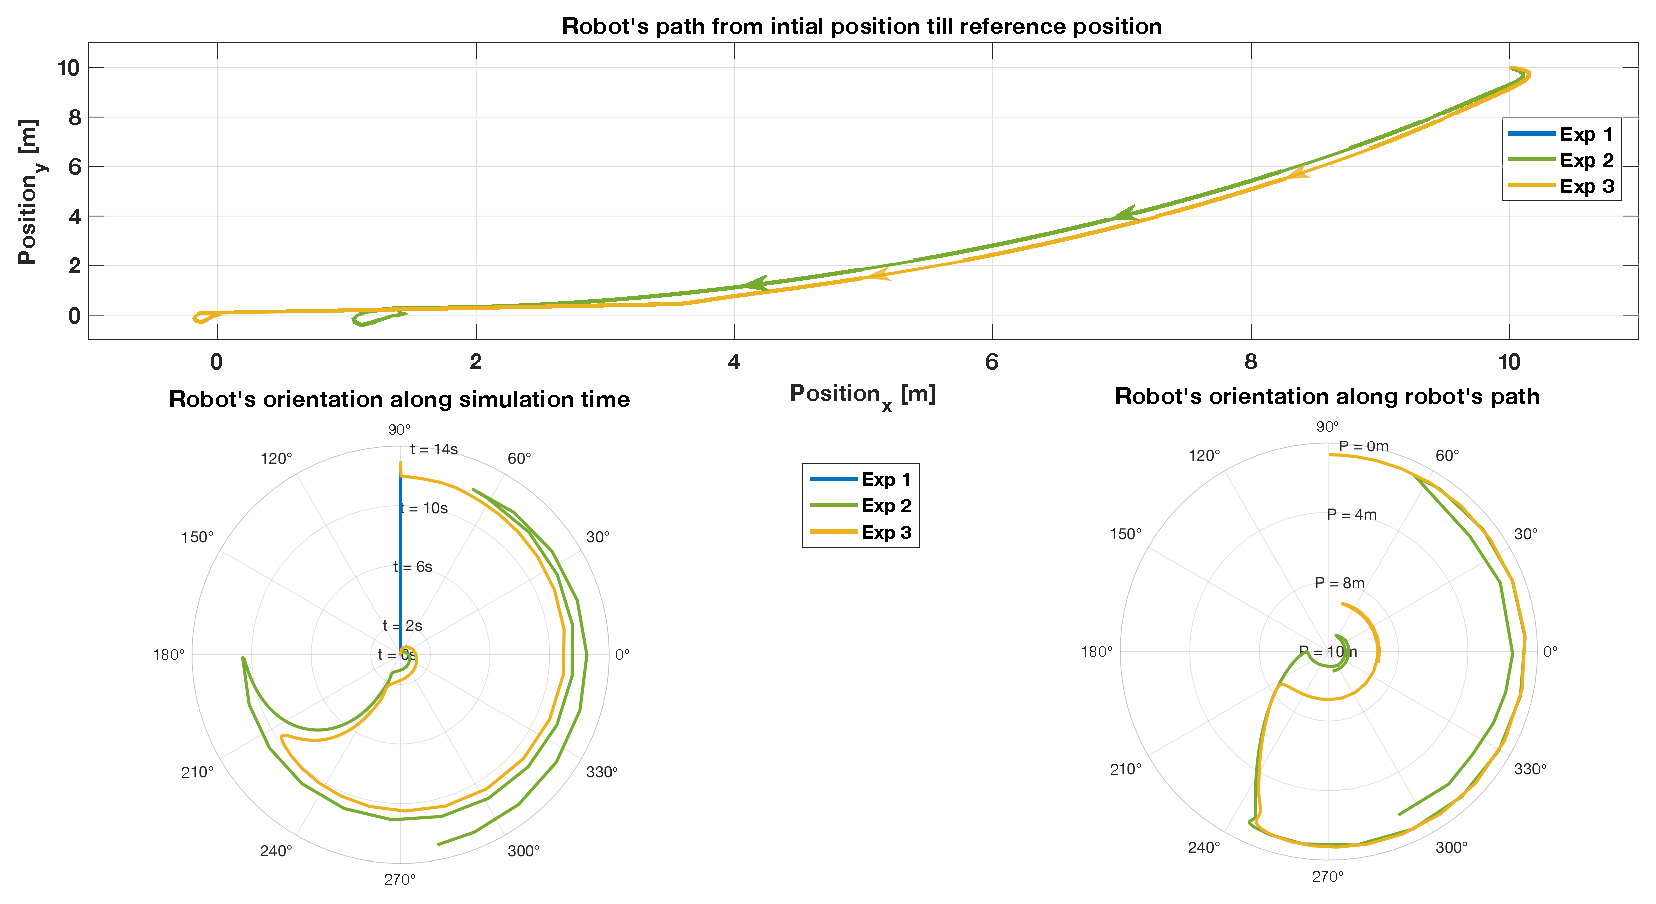
\includegraphics[scale=0.44]{pictures/graphs/sn1_states_2.eps}
 	\end{frame}
 	
 	\begin{frame}
 		\frametitle{Appendix B.2: Scenario \textrm{II} (Input Trajectory Evolution)}\label{b.2}
 		\centering
 		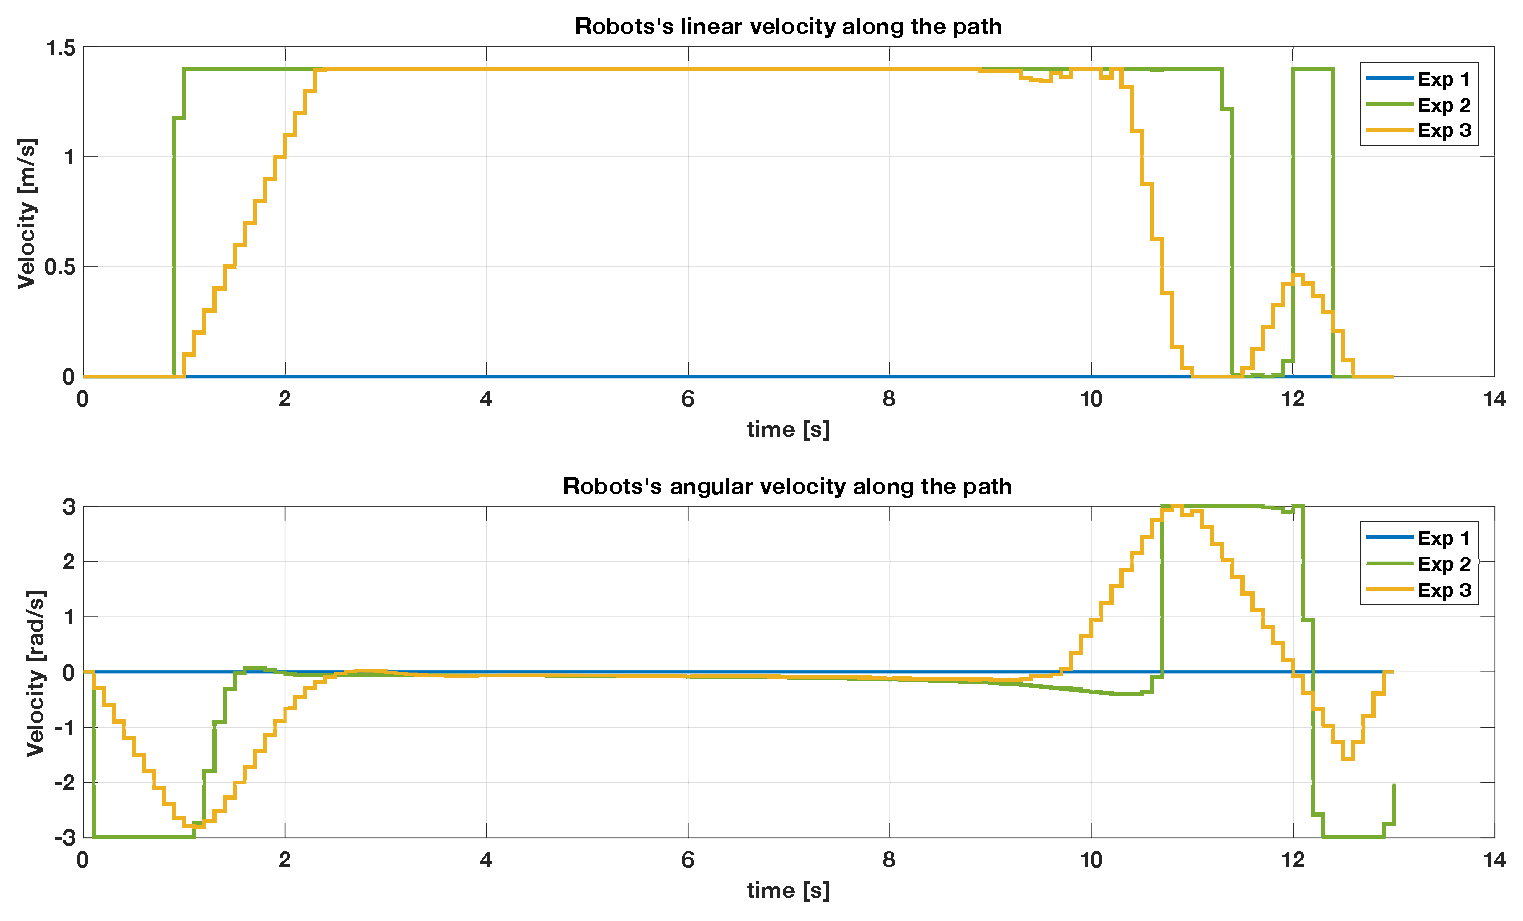
\includegraphics[scale=0.42]{pictures/graphs/sn1_inputs_2.eps}
 	\end{frame}
 
	\begin{frame}
		\frametitle{Appendix B.3: Scenario \textrm{II} (NMPC Computational Effort)}\label{b.3}
		\centering
		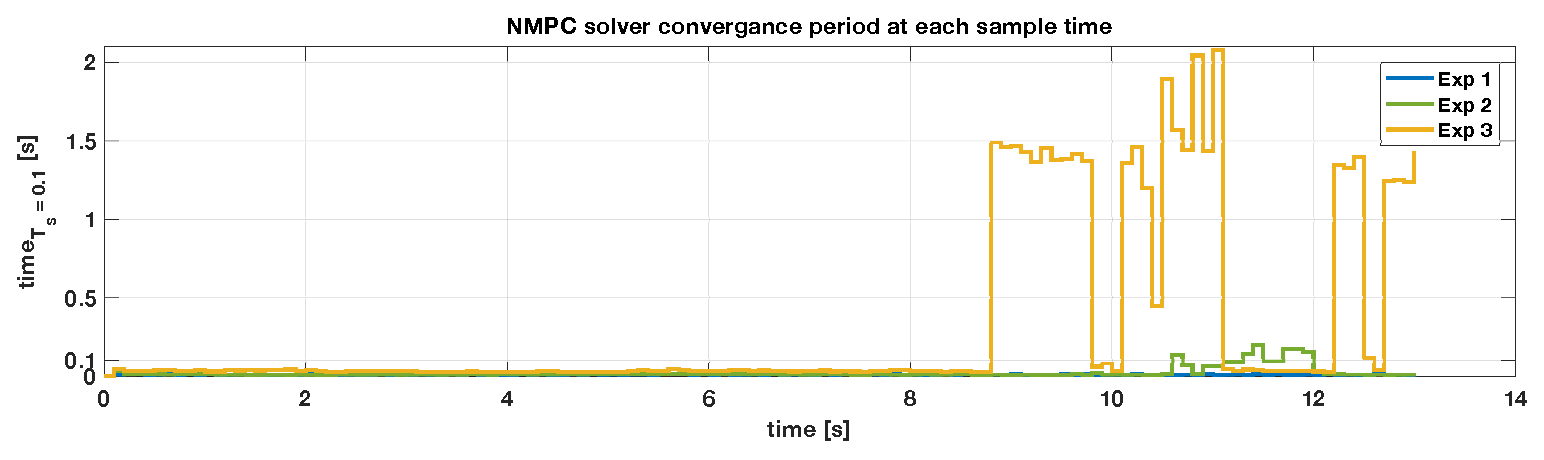
\includegraphics[scale=0.42]{pictures/graphs/sn1_solver_time_2.eps}
	\end{frame}

	\begin{frame}
		\frametitle{Appendix C.1: Scenario \textrm{III} (State Trajectory Evolution)}\label{c.1}
		\centering
		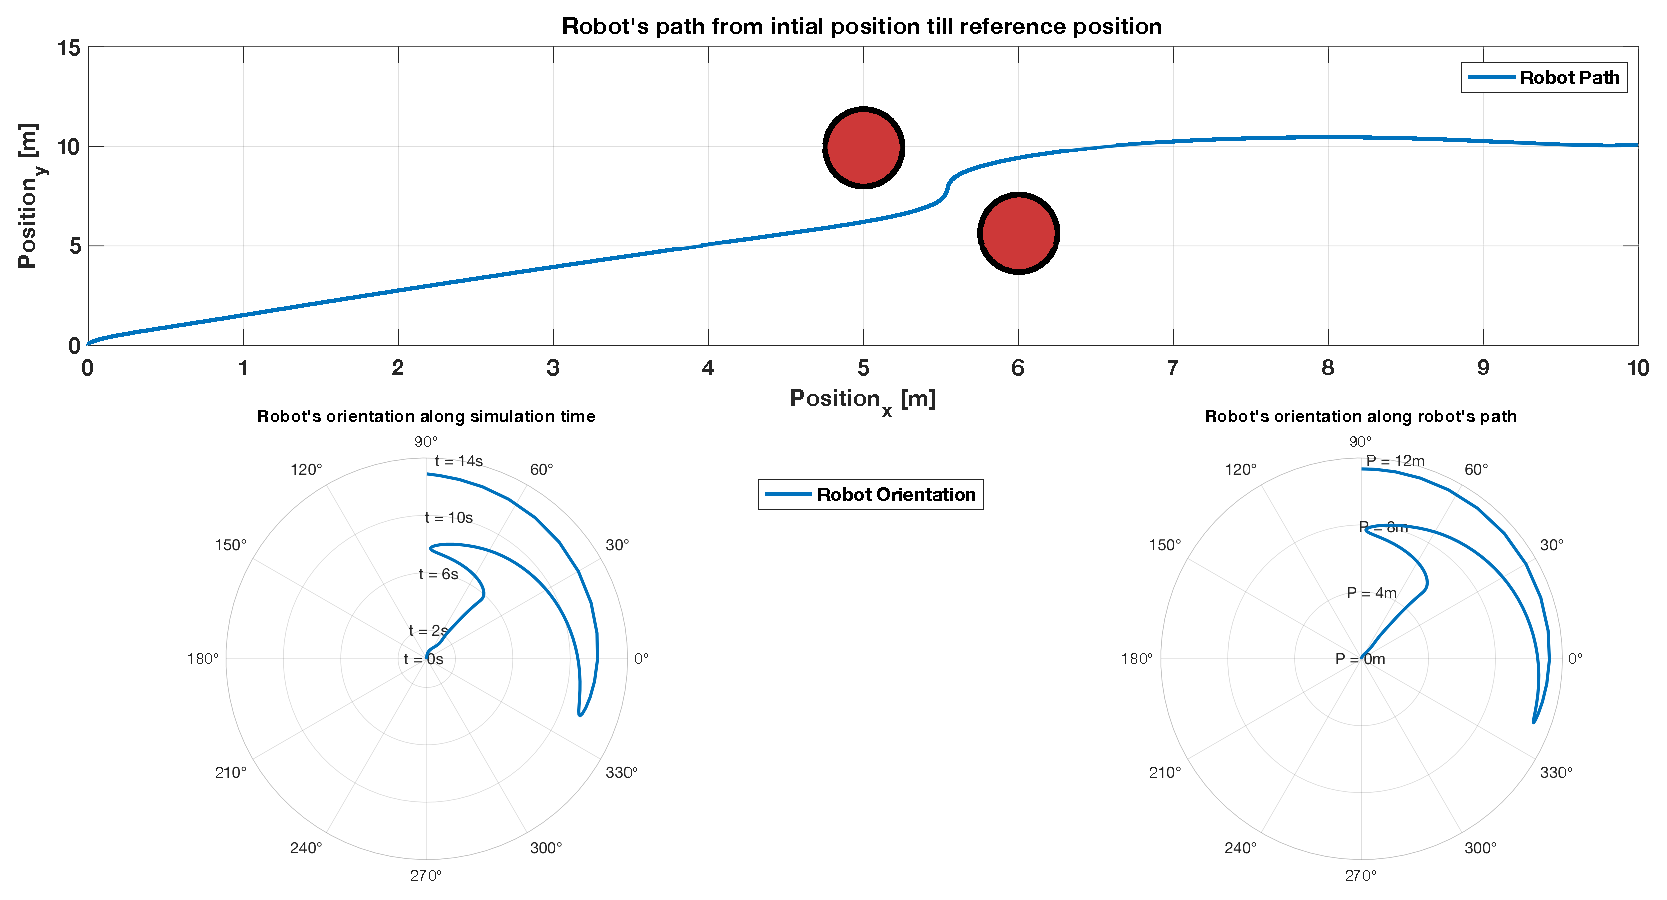
\includegraphics[scale=0.44]{pictures/graphs/sn2_states.eps}
	\end{frame}
	
	\begin{frame}
		\frametitle{Appendix C.2: Scenario \textrm{III} (Input Trajectory Evolution)}\label{c.2}
		\centering
		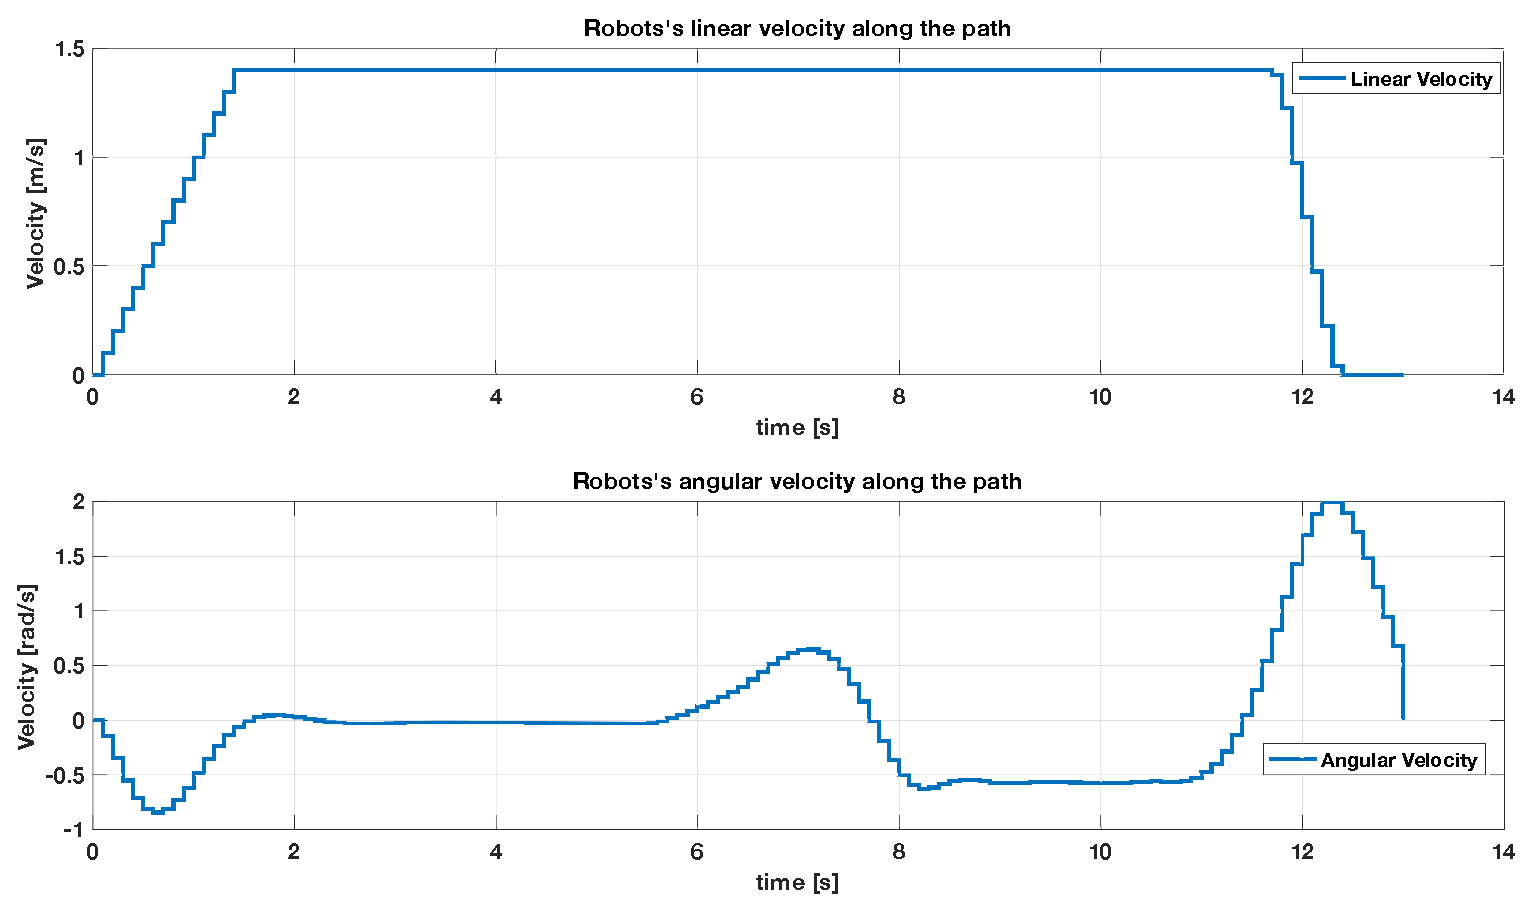
\includegraphics[scale=0.42]{pictures/graphs/sn2_inputs.eps}
	\end{frame}
	
	\begin{frame}
		\frametitle{Appendix C.3: Scenario \textrm{III} (NMPC Computational Effort)}\label{c.3}
		\centering
		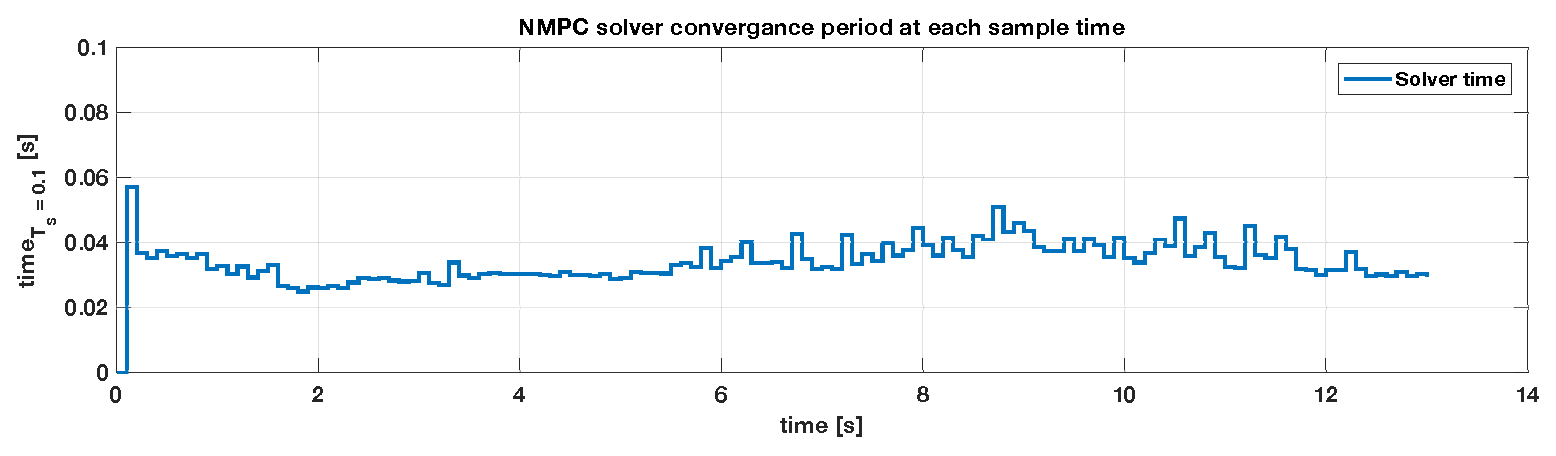
\includegraphics[scale=0.42]{pictures/graphs/sn2_solver_time.eps}
	\end{frame}
 
	\begin{frame}
		\frametitle{Appendix D: Scenario \textrm{II} (Robot Failure)}\label{d}
		\begin{columns}[T]
			\begin{column}{0.49\textwidth}
				\centering
				\includegraphics[scale=0.35]{pictures/robot_config_cart_mi.pdf}
			\end{column}
			\begin{column}{0.49\textwidth}
				\pause
				\centering
				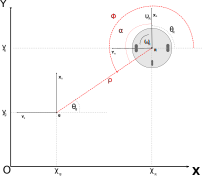
\includegraphics[scale=0.35]{pictures/robot_config_polar_mi.pdf}
			\end{column}
		\end{columns}
	\end{frame}
	
	
	
	%	\begin{frame}
	%		\frametitle{Scenario \textrm{IV}: Dynamic Environment}
	%		\begin{figure}[hbtp]
	%			\centering
	%			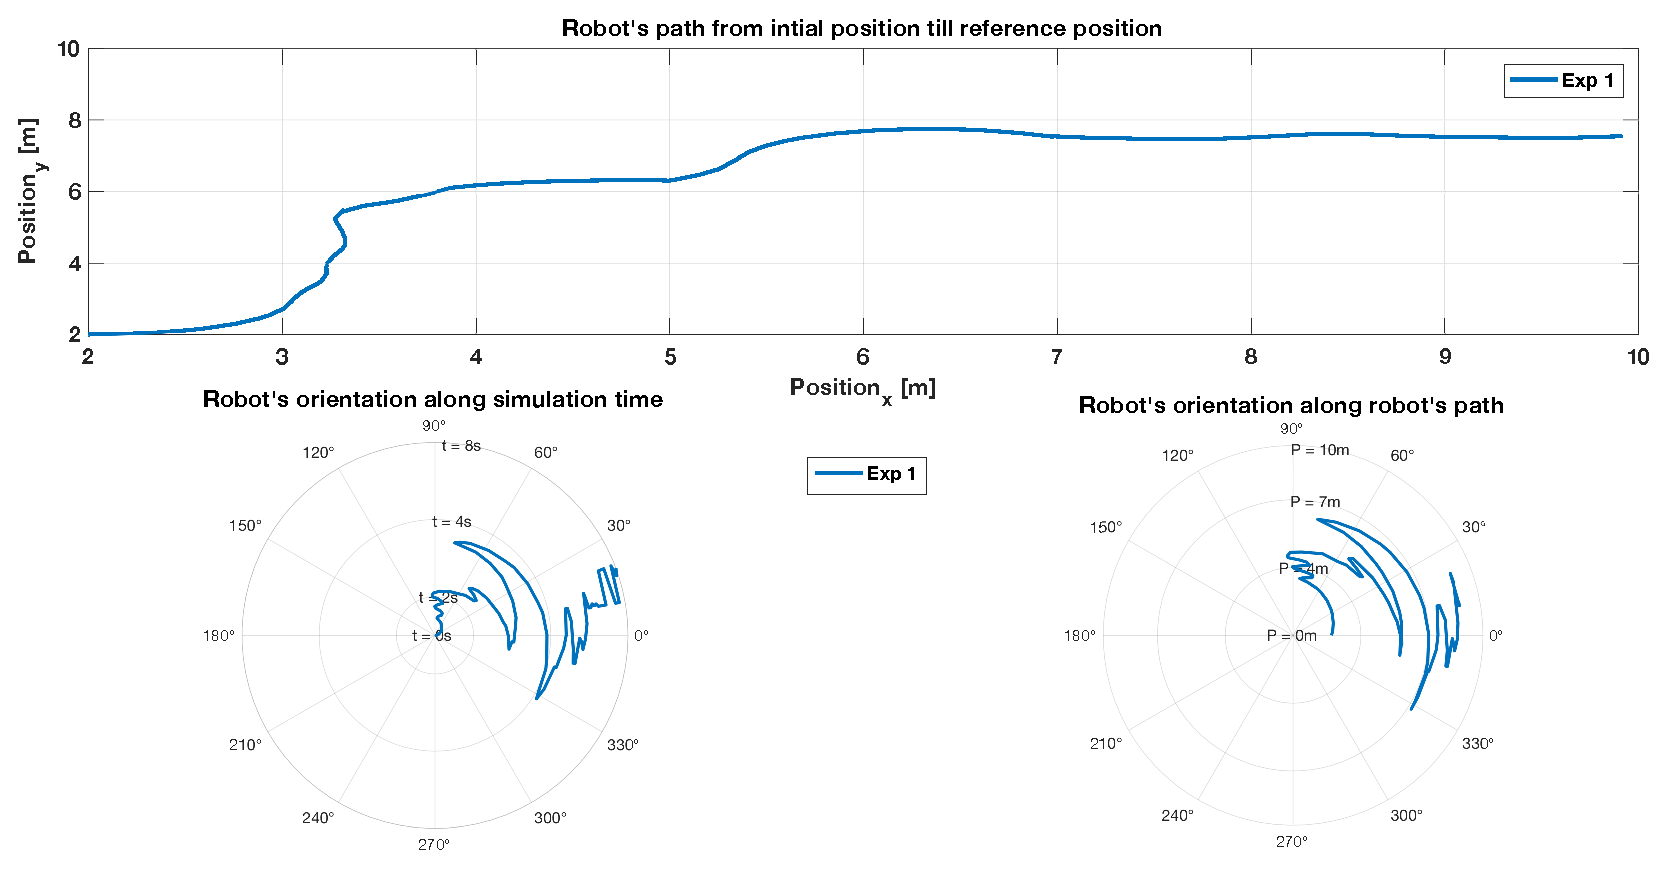
\includegraphics[scale=0.44]{pictures/graphs/sn3_states_1.eps}
	%			\caption{State Trajectory Evolution}
	%		\end{figure}
	%	\end{frame}
	%	
	%	\begin{frame}
	%		\frametitle{Scenario \textrm{IV}: Dynamic Environment}
	%		\begin{figure}[hbtp]
	%			\centering
	%			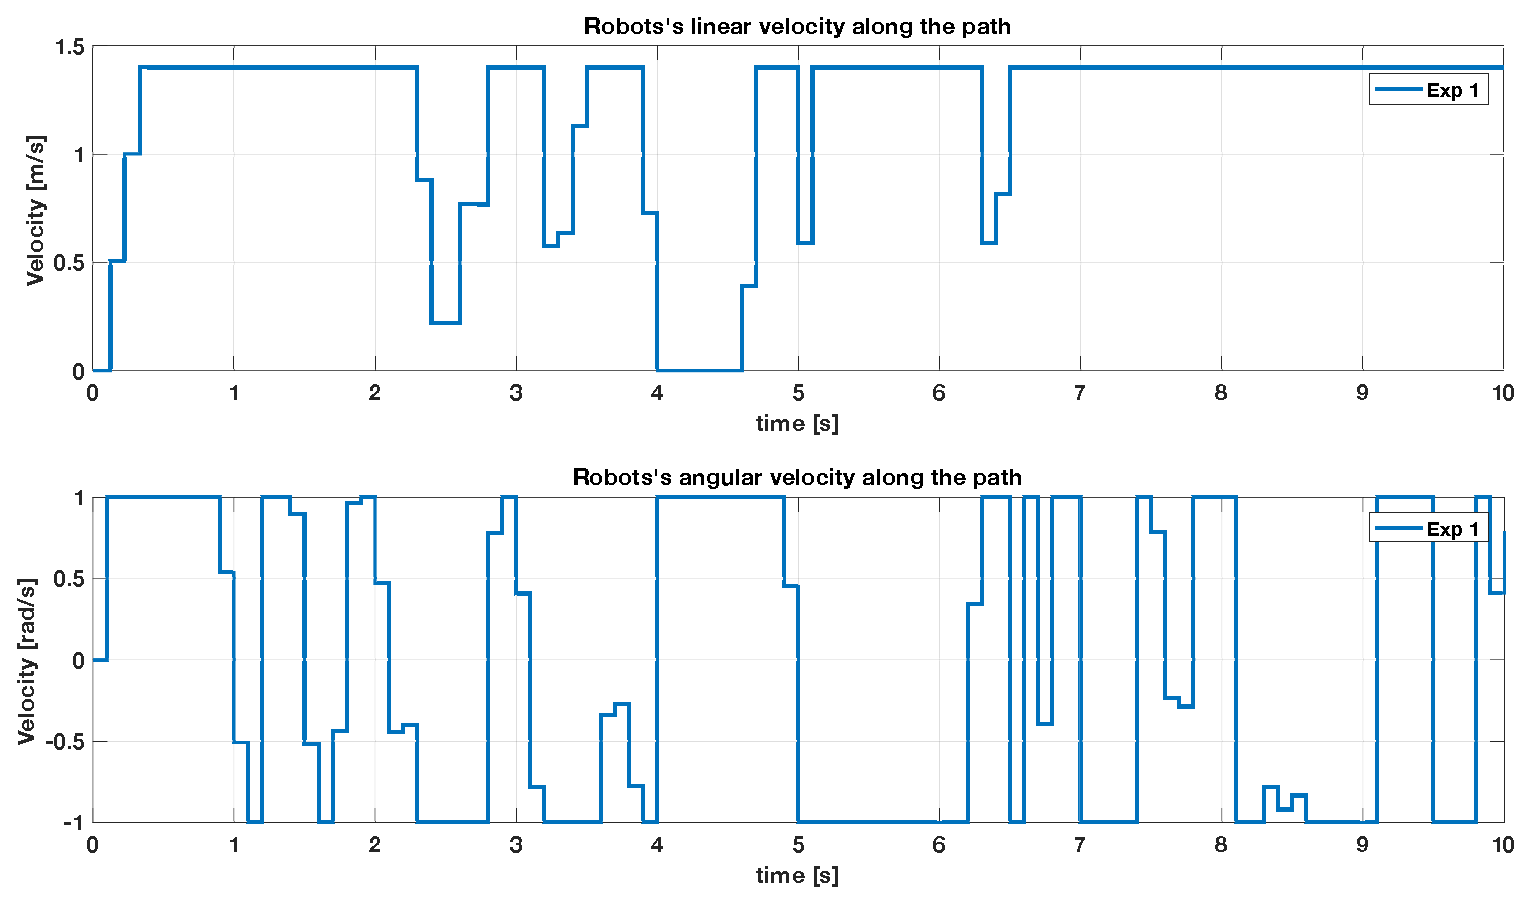
\includegraphics[scale=0.42]{pictures/graphs/sn3_inputs_1.eps}
	%			\caption{Input Trajectory Evolution}
	%		\end{figure}
	%	\end{frame}
	%	
	%	\begin{frame}
	%		\frametitle{Scenario \textrm{IV}: Dynamic Environment}
	%		\begin{figure}[hbtp]
	%			\centering
	%			\includegraphics[scale=0.42]{pictures/graphs/sn3_solver_time_1.eps}
	%			\caption{NMPC Computational Effort}
	%		\end{figure}
	%	\end{frame}
	
	